\section{Anwendungen der Ableitung}
\subsection{1. Ableitung}
Die 1. Ableitung beschreibt die Veränderung der Funktion $f$. Sie kann als Steigung der Kurventangente interpretiert werden.

Die 1. Ableitung macht somit Aussagen darüber, an welchen Stellen die Funktion wächst resprektive fällt:
\[
    f'(x_0) > 0: \hspace{2em} f \text{wächst beim Durchang durch den Punkt } P = (x_0,y_0)
\]
\[
    f'(x_0) < 0: \hspace{2em} f \text{fällt beim Durchang durch den Punkt } P = (x_0,y_0)
\]

\begin{center}
    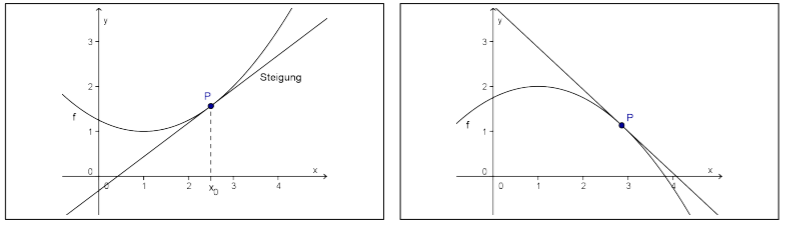
\includegraphics[width=1\linewidth]{images/ersteabl.png}
\end{center}

\subsection{2. Ableitung}
Die 2. Ableitung beschreibt die Veränderung der 1. Ableitung. Sie beschreibt das Krümmungsverhalten des Graphen.
\[
    f''(x_0) > 0: \hspace{2em} \text{Der Graph beschreibt eine Linkskurve}
\]
\[
    f''(x_0) < 0: \hspace{2em} \text{Der Graph beschreibt eine Rechtskurve}
\]
\begin{center}
    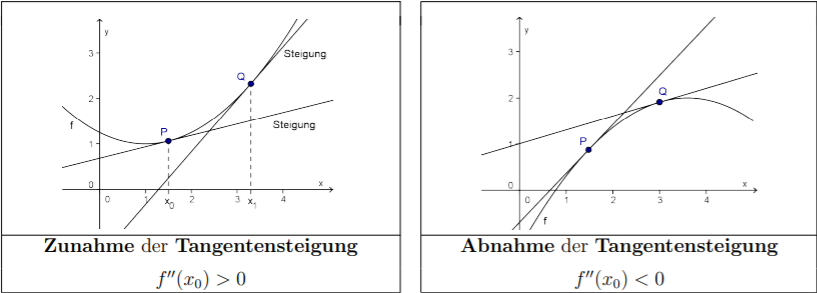
\includegraphics[width=1\linewidth]{images/zweiteabl.png}
\end{center}

\subsection{Beispiel}
\begin{center}
    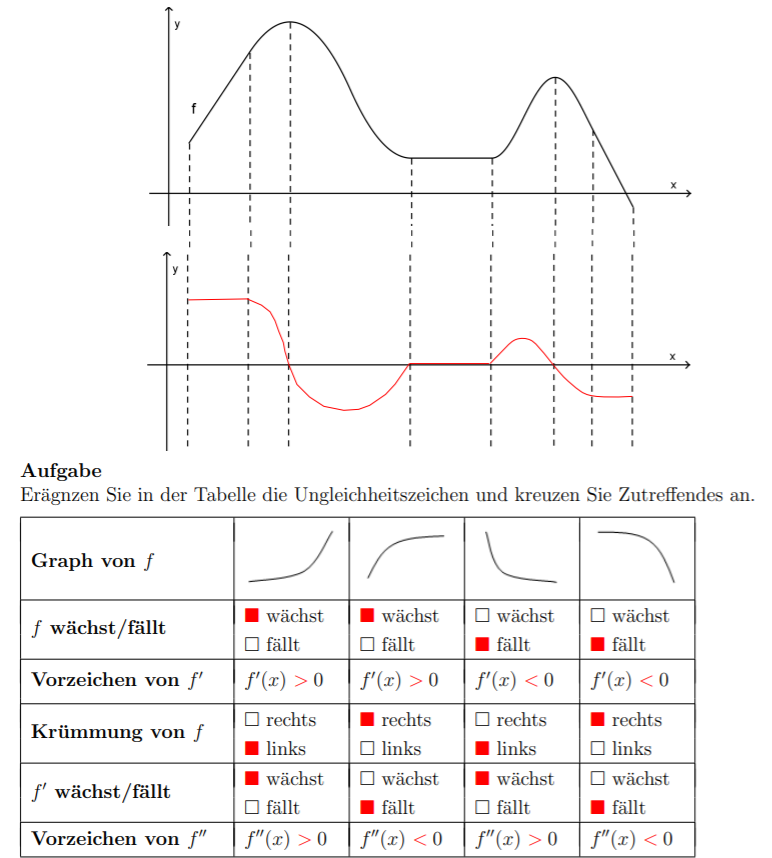
\includegraphics[width=1\linewidth]{images/ablbsp.png}
\end{center}

\subsection{Monotonie-Untersuchungen}
Für eine monoton wachsende, differenzierbare Funktion $f$ gilt: Ihre Steigung ($f'(x)$) ist $\geq 0$. Die Umkehrung ist ebenfalls richtig: Ist $f'(x) \geq 0$, so wächst $f$ monoton.

\subsubsection{Satz Monotonie}
$f'(x)$ ist auf einem Intervall überall $\geq 0 \Leftrightarrow f$ ist auf diesem Intervall monoton steigend. \\
$f'(x)$ ist auf einem Intervall überall $\leq 0 \Leftrightarrow f$ ist auf diesem Intervall monoton fallend.

\subsubsection{Beispiel Monotonie Aufgabe}
Gesucht: Alle monotonen Abschnitte der Funktion $f(x) = x^3 - 9x$
\begin{center}
    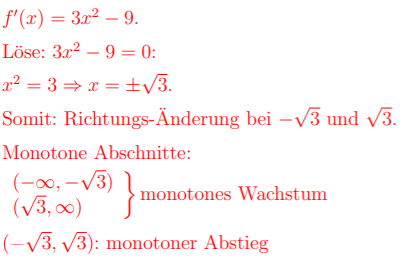
\includegraphics[width=0.4\linewidth]{images/monotonie.png}
\end{center}

\subsection{Relative Extrema}
Eine Funktion $f(x)$ besitzt an der Stelle $x_0$ ein relatives Maximum, wenn es eine Umgebung $U$ von $x_0$ gibt, so dass gilt $f(x) \leq f(x_0)$.

\begin{center}
    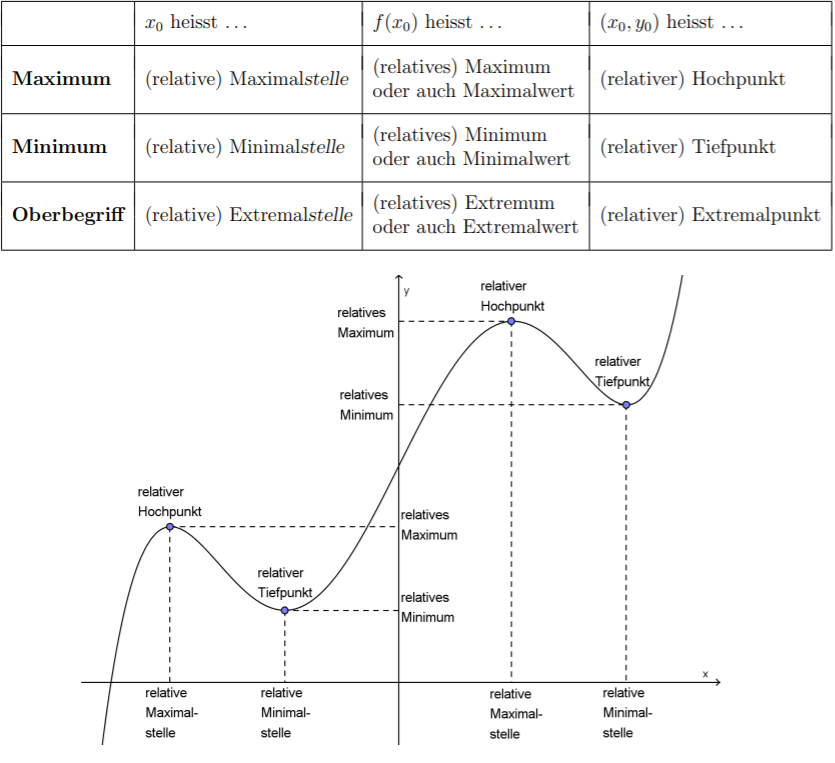
\includegraphics[width=1\linewidth]{images/rel.png}
\end{center}

\subsubsection{Randpunkte}
Ein abgeschlossenes oder halboffenes Intervall besitzt Randpunkte:
\begin{enumerate}
    \item $[a,b)$: Randpunkt $a$
    \item $(a,b]$: Randpunkt $b$
    \item $[a,b]$: Randpunkte $a,b$
\end{enumerate}
Die Punkte eines Intervalls, die keine Randpunkte sind, heissen innere Punkte von I.

\subsubsection{Kandidaten für relative Extrema}

\begin{center}
    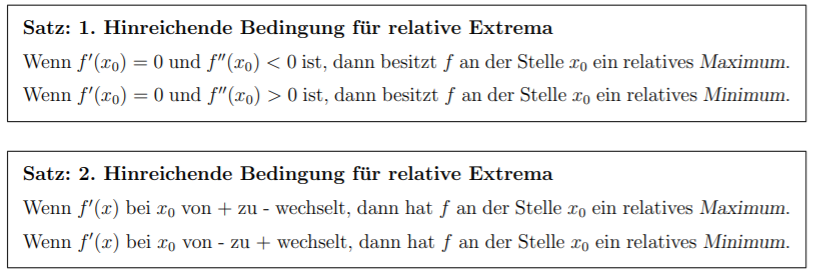
\includegraphics[width=1\linewidth]{images/rel_extrem.png}
\end{center}

\begin{center}
    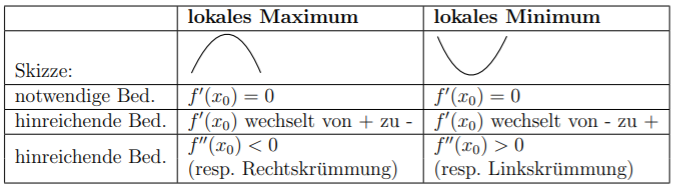
\includegraphics[width=1\linewidth]{images/rel2.png}
\end{center}

\begin{center}
    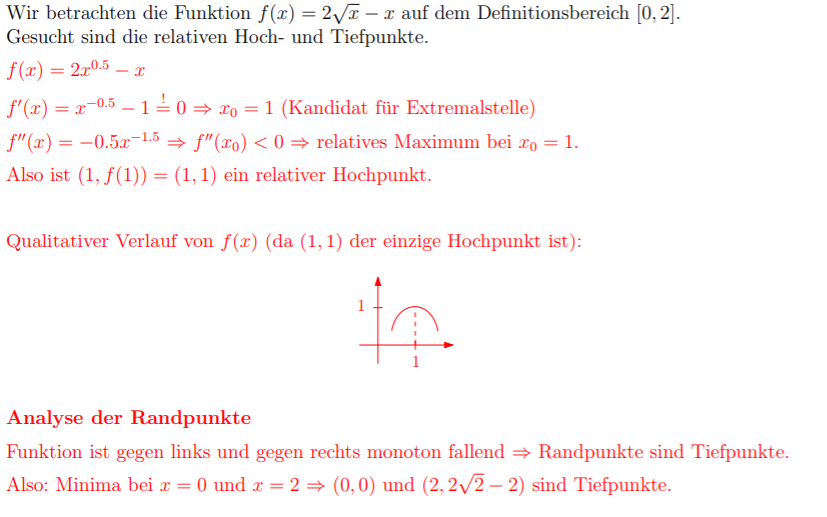
\includegraphics[width=1\linewidth]{images/relbsp.png}
\end{center}
\vfill
\subsection{Wendepunkte und Sattelpunkte}
Punkte, an denen sich das Krummungsverhalten des Graphen ändert (d.h. bei denen eine Linkskurve in eine Rechtskurve übergeht oder umgekehrt), heissen Wendepunkte. Wendepunkte mit horizontaler Tangente heissen Sattelpunkte.
\begin{center}
    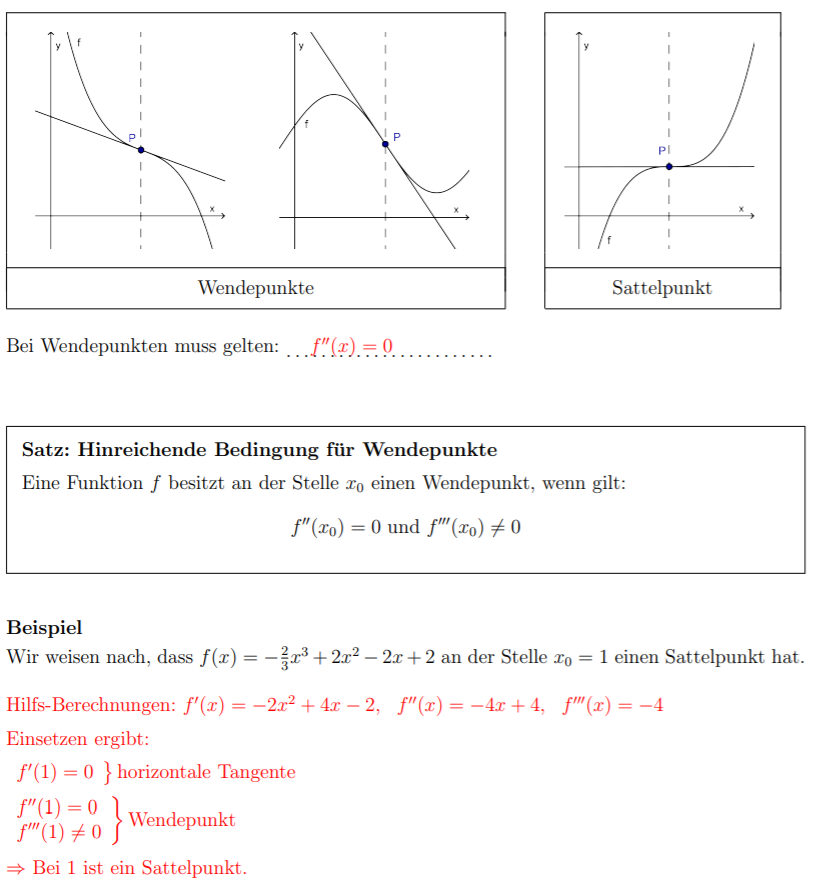
\includegraphics[width=1\linewidth]{images/wendepunkt.png}
\end{center}

\subsubsection{Deutung von Extrema und Wendepunkten}
\begin{center}
    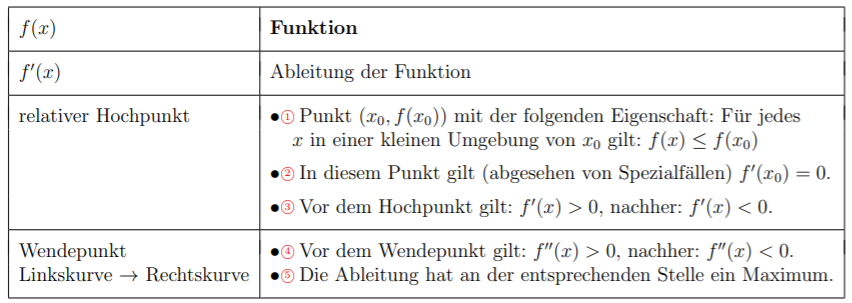
\includegraphics[width=1\linewidth]{images/deutungwendepunkte.png}
\end{center}

\subsection{Kurvendiskussion}
\begin{center}
    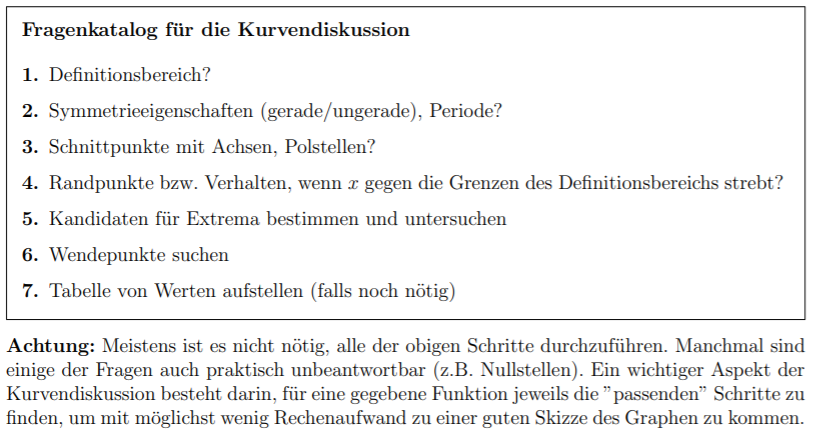
\includegraphics[width=1\linewidth]{images/kurvendiskussion_fragekatalog.png}
\end{center}

\begin{center}
    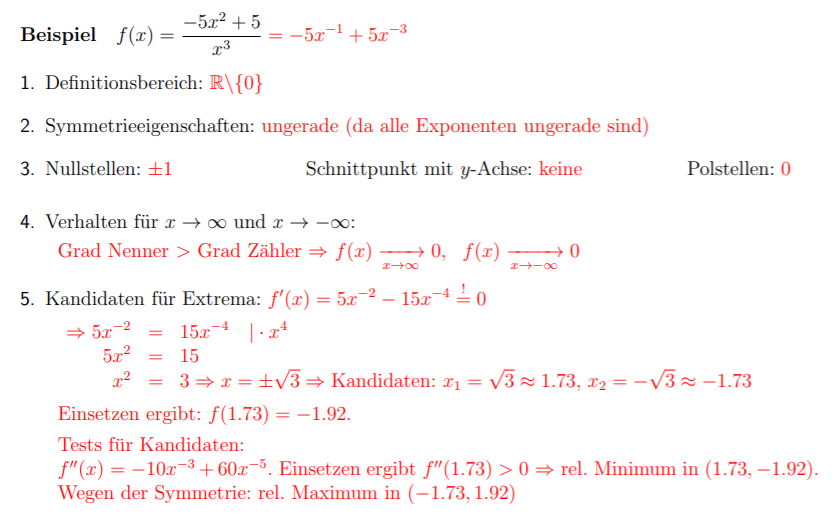
\includegraphics[width=1\linewidth]{images/kurvbsp.png}
\end{center}

\begin{center}
    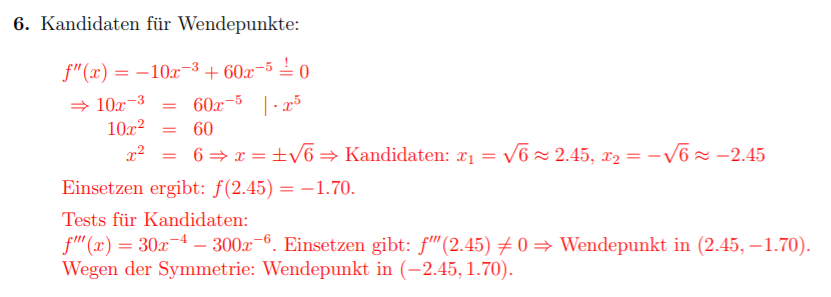
\includegraphics[width=1\linewidth]{images/kurvbsp2.png}
\end{center}

\subsection{Extremwertaufgaben}

\begin{center}
    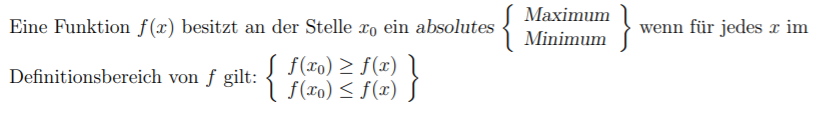
\includegraphics[width=1\linewidth]{images/minmax.png}
\end{center}

\begin{center}
    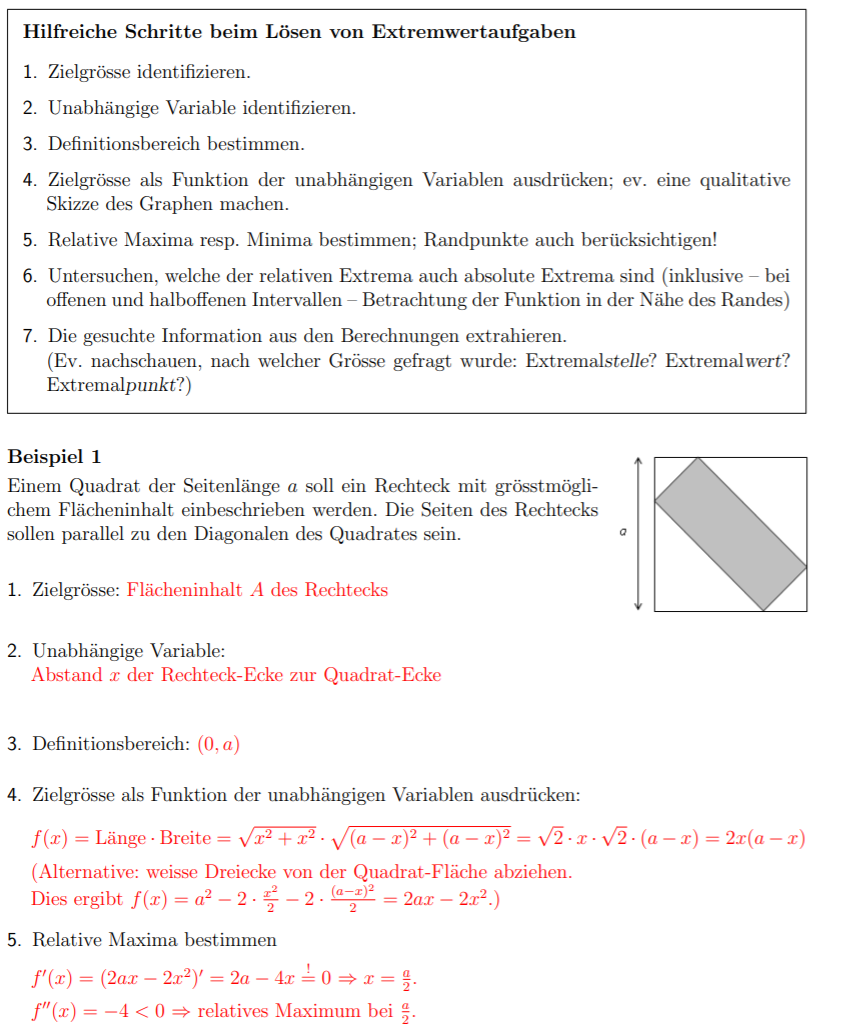
\includegraphics[width=1\linewidth]{images/extrem.png}
\end{center}

\begin{center}
    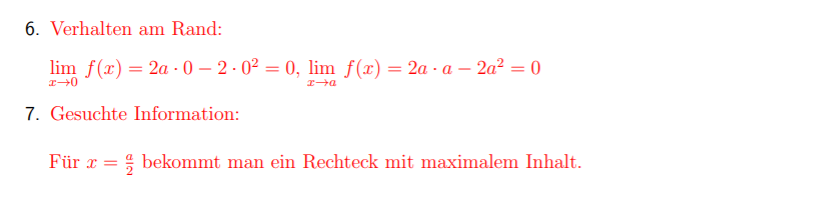
\includegraphics[width=1\linewidth]{images/extrem2.png}
\end{center}
\vfill
\begin{center}
    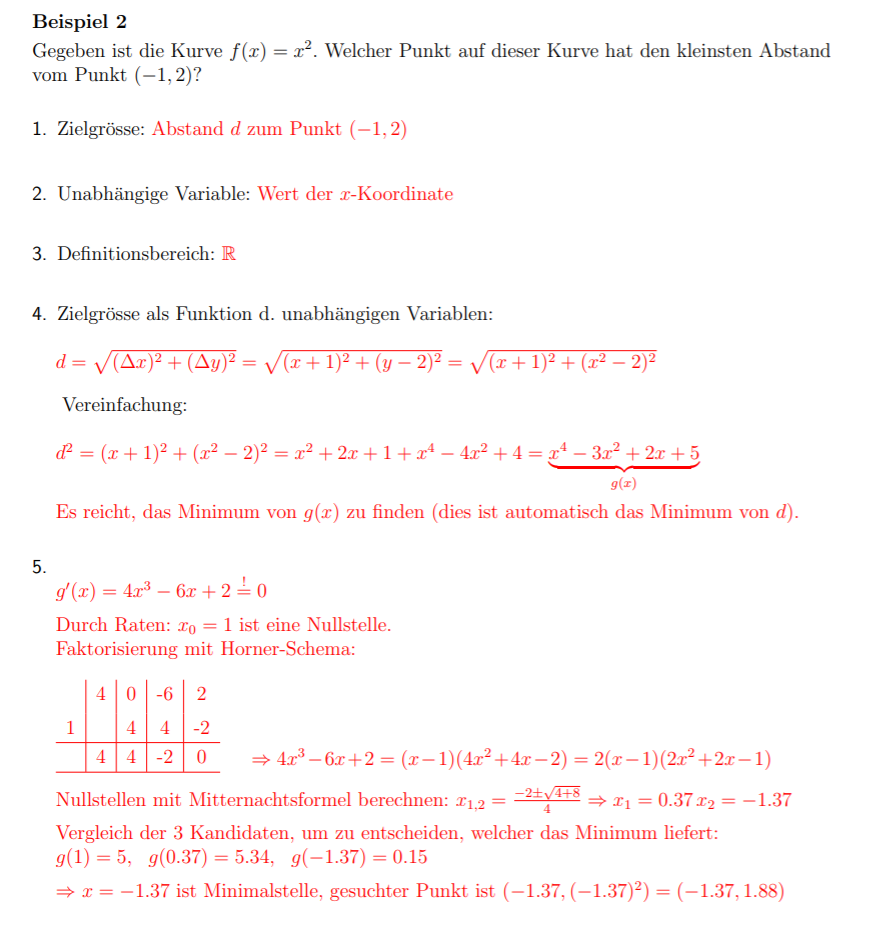
\includegraphics[width=1\linewidth]{images/extrem3.png}
\end{center}